% $Id: report.tex,v 1.7 2007-09-12 10:13:56 ajohan Exp $
\documentclass{article}
\usepackage{graphicx}
\usepackage{bm,url}
\graphicspath{{./fig/}{./png/}}
\input apj
\title{Pencil Code User Meeting 2007\footnote{This meeting
was sponsored by Nordita and the European Science Foundation (ESF)}\\
(Stockholm, 14-17 August)}
\author{Organizers: Axel Brandenburg, Boris Dintrans, Wolfgang Dobler,\\
Anders Johansen, \& Petri K\"apyl\"a}
\date{\today,~ $ $Revision: 1.7 $ $}
\begin{document}
\maketitle

\section{Summary} % (up to 1 page)

This was the third meeting of this kind which brought together
some 19 Pencil Code users from around the world including
Calgary, Cambridge, Freiburg, Halifax, Heidelberg, Helsinki,
London, Potsdam, Stanford, Stockholm, Toulouse, and Uppsala.
The program of the 4 day meeting included 19 talks of about
30+15 minutes with science results and 9 discussion sessions
where a number of emerging issues were considered.
Some of the scientific highlights include presentations about
the co-evolution of dust and gas in magnetized self-gravitating
shearing sheets, the introduction of curvilinear coordinates,
hydrodynamic and hydromagnetic simulations of
Taylor-Couette flows in cylindrical coordinates,
the implementation of an implicit solver of the heat equation and
of a multigrid solver for the Poisson equation.
The discussion topics included in particular
the anticipated migration from CVS to the subversion repository,
the change to version 3 of the GPL license agreement,
improvements of the suite of automatic nightly tests of the code,
improvements of the manual,
a multi-author paper discussing methods and tests,
as well as discussions about curvilinear coordinate systems
and the option of using upwinding derivatives in
cartesian and non-cartesian coordinate systems.
All talks are recorded and now publicly available as streaming videos; see
\url{http://agenda.albanova.se/conferenceDisplay.py?confId=185}.

\section{Description of the scientific content and discussion at the event}

The purpose of the meeting was to bring the core developers together and
to allow others to interact with them and learn more about the Pencil Code
(http://www.nordita.dk/software/pencil-code/). The code is a multipurpose
code for massively parallel computing (especially on the cheaper
Linux cluster). It includes optionally hydrodynamics, magnetic fields,
radiation, ionization, multi-species dust dynamics with coagulation, dust and
tracer particles, self-gravity, and
certain reaction-diffusion equations. It is developed and maintained under
the Concurrent Versioning System (CVS; see http://www.nongnu.org/cvs/)
by around 25 people with check-in permission and has been downloaded by
over 450 registered users (without check-in permission).

During the meeting it became clear that
the {\sc Pencil Code} has expanded significantly in the number of
lines of code and the number of subroutines (Fig.~\ref{pfile-size}).
The increase in the functionality of the code is documented by the
rise in the number of sample problems (Fig.~\ref{pauto-tests}).
In order to keep the development of the code going, it it important
that the users are able to understand and modify (program!) the code.

\begin{figure}[htb]
  \centering
  \includegraphics%
    [width=.6\textwidth,keepaspectratio]%
    {pfile-size}
  \caption{Number of lines of code and the number of subroutines
  since the end of 2001. The jump in the Summer of 2005 was the
  moment when the developments on the side branch (eos branch) were
  merged with the main trunk of the code. Note the approximately
  linear scaling with time.}
  \label{pfile-size}
\end{figure}

\begin{figure}[htb]
  \centering
  \includegraphics%
    [width=.6\textwidth,keepaspectratio]%
    {pauto-tests}
  \caption{Number of tests in the sample directory that are
  used in the nightly auto tests. Note again the approximately
  linear scaling with time.}
  \label{pauto-tests}
\end{figure}

\section{Assessment of the results and impact of the event on the future
direction of the field}

The meeting had been important for a number of reasons.
Given that there was a large number of new users, this meeting
helped introducing these new users to each other and to the
rest of the core developers.
Some of the new users emphasized the usefulness of the manual,
but they identified also a number of shortcomings having to do
with learning the interior of the code and being able to modify it.
As a consequence, a number of modifications have already been made
in the manual.

Another important development is the imminent migration of the
CVS repository to subversion (SVN). During the meeting this
process was tested and the code is now available on a preliminary
SVN server.
The final migration will be done in a few weeks when all other
users had a chance to test the new system and to identify problems.
By and large, the problems (e.g.\ with firewalls) are minor in comparison
with the advantages (moving files, preserving links, and the atomic
version numbers that help tracing the order of changes in various
routines).

As part of the new SVN repository, there is now also a
new bug tracking system (Trac).
Until now we have been using bugzilla instead, but now the
entire bugzilla database has been moved to Trac.
Bugs are now referred to as tickets, emphasizing that much
of it is rather a request for improvement.
A new additional tickets have been filed and several
additional clean-ups in the code have already been done.

On the technical side, a major addition to the code has been the
implementation of curvilinear coordinates.
In the Pencil Code this became a relatively simple modification,
because this change is simply represented by going from
partial derivatives to covariant derivatives.
This implies the addition of terms involving Christoffel symbols
and emerges as a relatively neat modification.
During the meeting it was emphasized that some of the recent
additions done for spherical coordinates may still be missing
for cylindrical coordinates (e.g.\ timestep control and some
diagnostic variables).
The implementation of high-order upwinding was regarded as
a useful option that seemed to require a lot of work.
This is because high-order upwinding corresponds to
the addition of a hyperviscosity term with an amplitude
proportional to the magnitude of the velocity, and hyperviscosity
would be cumbersome to implement in spherical or cylindrical
coordinates.
However, it was then realized that such a change might be
relatively simple because the change to curvilinear coordinates
corresponds also here for first order derivatives just to the addition
of relatively few additional terms involving Christoffel symbols.

\section{Highlights of results obtained with Pencil Code during the last year}

\subsection{Planetesimal formation by self-gravity}

\begin{center}
  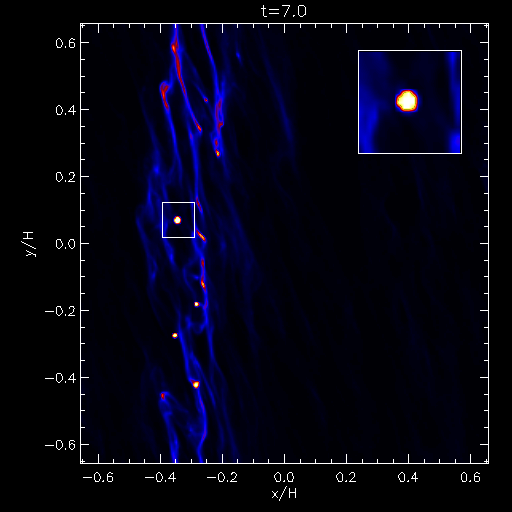
\includegraphics[width=0.5\linewidth]{planetesimal.png}\\
\end{center}
A self-gravity solver was implemented for the Pencil Code by Anders Johansen
and Jeff Oishi as part of an exchange programme between Max Planck Institute for
Astronomy in Heidelberg and American Museum of Natural History in New York.
This solver was subsequently used for modelling the gravitational instability
of solids (boulders) in a protoplanetary disc. The figure shows the column
density of solids. Boulders have concentrated in the magnetised turbulence into
a thin sheet with a so high density that gravitationally bound objects have
condensed out of the turbulent flow.

\section{Final program of the meeting}

\begin{verbatim}
Tuesday, 9-10:30, 11-12:30
9:00 Axel Brandenburg   Introduction
9:15 Anders Johansen    Dust in self gravitating shearing sheets
Cristina Green          Traveling waves in sheared convection
Discussion

Tuesday, 14-15:30, 16-17:30
Wolfgang Dobler         CVS, Mercurial or Subversion -- do we need a
Sven Bingert            Field aligned heat conduction in the corona
Marcus Gellert          Hydrodynamic simulations in cylindrical coordinates
Discussion

Wednesday, 9-10:30, 11-12:30
Miikka Väisälä          Formation of elephant trunks
Tobias Heinemann        Migrating to subversion
Discussion

Wednesday, 9-10:30, 11-12:30
Steve Berukoff          Plans to implement protostellar disc chemistry
Chao-Chin Yang          Fueling the circum-nuclear region of a barred galaxy
Discussion

Wednesday, 14-15:30, 16-17:30
Petri Käpylä            Hi-res MHD on the Finnish Louhi machine
Anne Liljeström         Reynolds stresses in shearing boxes
Discussion

Thursday, 9-10:30, 11-12:30

Dhrubaditya Mitra       Simulations in spherical coordinates
Nathalie Toque          Turbulent diffusion
Boris Dintrans          I. Global convection; II. Implicit method
Discussion

Thursday, 14-15:30, 16-17:30

Wladimir Lyra           Global disc simulations
Lars Mattsson           Disc Simulations: Evolving Late-type Galaxies
Mikaela Sundberg        Code comparison projects - A sociological view
Discussion

Friday, 9-10:30, 11-12:30

Wolfgang Dobler         Multigrid solvers for the Pencil Code
Discussion

Friday, 14-15:30

Axel Brandenburg        Parallelization in the x-direction
Discussion
\end{verbatim}

\section{Budget}


\includegraphics[width=4cm]{140px-Logo-a}

\includegraphics[width=3cm]{logo_esf}

\vfill\bigskip\noindent\tiny\begin{verbatim}
$Header: /var/cvs/brandenb/f90/pencil-www/UserMeetings/2007/report.tex,v 1.7 2007-09-12 10:13:56 ajohan Exp $
\end{verbatim}

\end{document}
